\documentclass[12pt]{article}
\usepackage{graphicx} % Required for inserting images
\usepackage{multicol}
\usepackage{amsmath}
\usepackage{gvv-book}
\usepackage{gvv}


\title{\textbf{2.10.33}}
\author{\textbf{Aditya Appana - EE25BTECH11004 }}
\date{September 8, 2025}

\begin{document}

\maketitle

\section*{Question}

Let $\alpha , \beta, \gamma$ be distinct real numbers. The points with position vectors $\alpha\hat{i} + \beta\hat{j} + \gamma\hat{k}$, $\beta\hat{i} +\gamma\hat{j} + \alpha\hat{k}$, $\gamma\hat{i} + \alpha\hat{j} + \beta\hat{k}$

\begin{enumerate}\begin{multicols}{2}
    \item are collinear
    \item form an equilateral triangle
    \item form a scalene triangle
    \item form a right angled triangle
    \end{multicols}
\end{enumerate}

\section*{Solution}

Let $\vec{A}$ be \myvec{\alpha \\ \beta \\ \gamma}, $\vec{B}$ be \myvec{ \beta \\ \gamma \\ \alpha}, and $\vec{C}$ be \myvec{\gamma \\ \alpha \\ \beta}. 

First, we need to check when the three points are collinear. We can do this using the collinearity matrix: \begin{align}\myvec{\vec{C}-\vec{A} & \vec{B} - \vec{A}}^T\end{align}If the rank of the matrix is 1, then the points are collinear.

\begin{align}
\myvec{\gamma - \alpha & \alpha - \beta & \beta - \gamma \\ \beta - \alpha & \gamma - \beta & \alpha - \gamma}
\end{align}

The rank of this matrix will be 1 only when all the elements in the bottom row of the matrix are equal to 0. This occurs only when $\alpha = \beta = \gamma$, which contradicts the fact that $\alpha, \beta, \gamma$ are distinct.\\

Therefore the points must be non-collinear and form a triangle.\\

The sides of the triangle are $\vec{A} - \vec{B}, \vec{B} - \vec{C}, \vec{C}- \vec{A}$.\\

\begin{align}
\vec{A-B} = \myvec{\alpha - \beta \\ \beta - \gamma \\ \gamma - \alpha} \\
\vec{B-C} = \myvec{\beta - \gamma \\ \gamma - \alpha \\ \alpha - \beta} \\
\vec{C-A} = \myvec{\gamma - \alpha \\ \alpha - \beta \\ \beta - \gamma}
\end{align}


$\norm{\vec{A}-\vec{B}} = \norm{\vec{B}-\vec{C}} = \norm{\vec{C}-\vec{A}} = \sqrt{(\alpha - \beta)^2  + (\beta - \gamma)^2 + (\gamma - \alpha)^2}$ 

The three points therefore form an \textbf{equilateral triangle}, so option (2) is correct.

For example, let us take $\alpha = 2$, $\beta = 1$, $\gamma = 3$.
We get an equilateral triangle as shown below:

\begin{figure}[H]
    \centering
    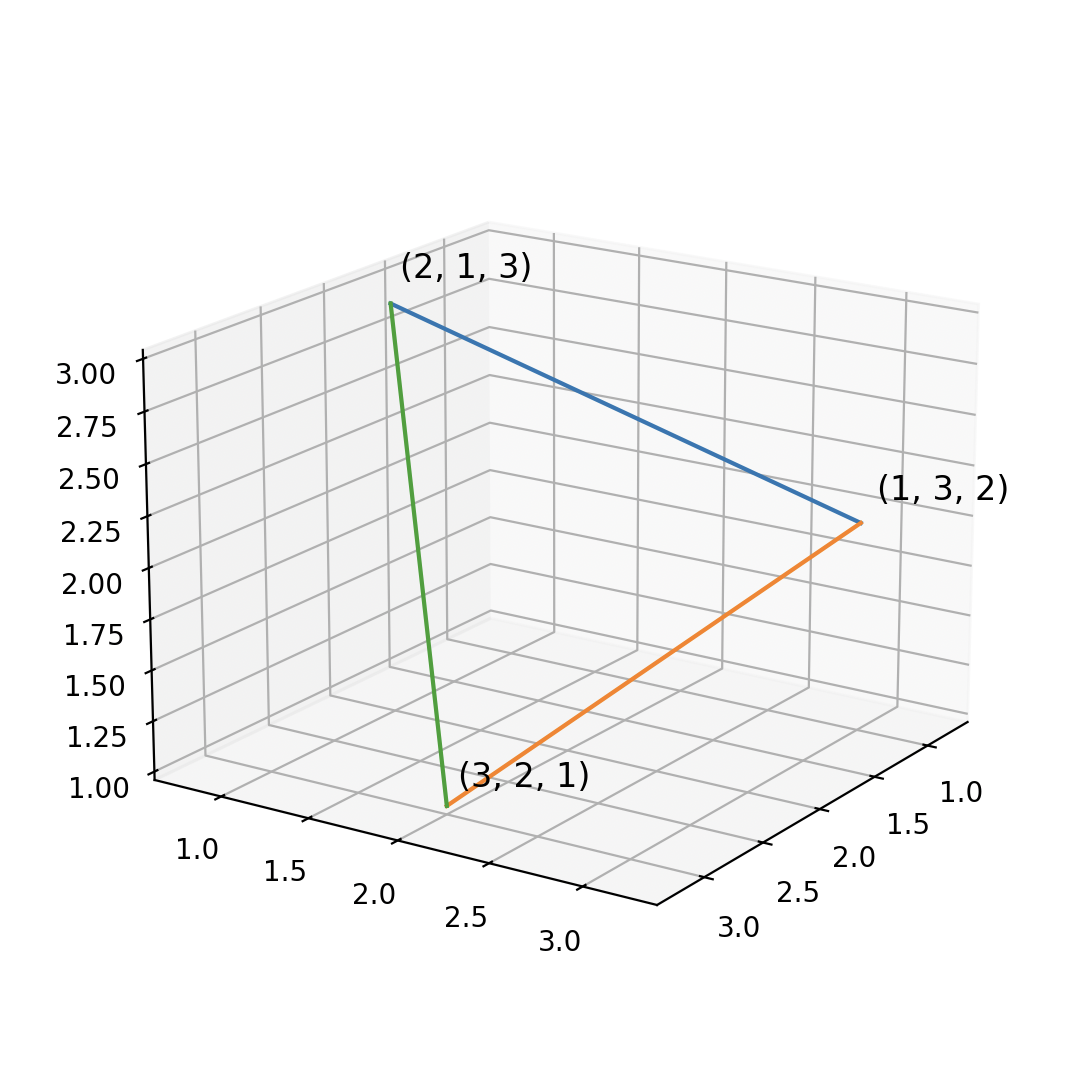
\includegraphics[width=0.7\columnwidth]{Figs/Example.png}
    \caption{Equilateral Triangle}
    \label{fig:placeholder}
\end{figure}



\end{document}

